\clearpage

\section{Diffusion models}\label{sec:Diffusion}\index{denoising diffusion}\index{diffusion model}

\begin{notebox}
\textbf{Paper: } \fullcite{ho_denoising_2020}
\vspace{5pt}

\href{https://proceedings.neurips.cc/paper/2020/hash/4c5bcfec8584af0d967f1ab10179ca4b-Abstract.html}{reviews}
\hspace{1cm}
\href{https://github.com/hojonathanho/diffusion}{code}
\hspace{1cm}
\href{run:/home/magda/Dropbox/Zot/Ho et al_2020_Denoising Diffusion Probabilistic Models.pdf}{Local pdf}
\vspace{3pt}

Read with Simon on 27/1/2022
\hfill Notes taken: 13/2/2022 \index{February 2022}
\end{notebox}

\begin{notebox}[colback=red!5]
\tldr Diffusion process is a Markov chain gradually adding small quantities of noise to the data until the signal is completely destroyed - seems as random noise. 
The diffusion model is trained to reverse this process.
When the diffusion consists of Gaussian noise, the sampling transitions can be Gaussian as well.
The diffusion (forward) process is seen as a posterior $q(\rvx_{t} \vert \rvx_{t-1})$ of the reverse model $p_{\theta}(\rvx_{t-1} \vert \rvx_{t})$.
Here, however, the posterior is fixed (Gussians with variance schedule) so that the full chain $\rvx_{1:T}$ can be generated from the data $\rvx_0$ and the model is then trained to get back using variational lower bound on $\log p_{\theta}(\rvx_0)$ as the loss. The trick is in rewriting the lower bound so that it is trainable. It all relies on tractability of the conditionals because they are all Gaussians.
\end{notebox}

\begin{notebox}[colback=yellow!5]
\textbf{Notes:} 
\begin{itemize}[nosep]
\item What if the Markov chain was not Gaussian? Would it still be possible to find a tractable solution and would it be good for anything?\index{idea} Probably not. The initial generative noise would then be non-Gaussian - so what?
\end{itemize}
\end{notebox}


\begin{figure}[ht]
\centering
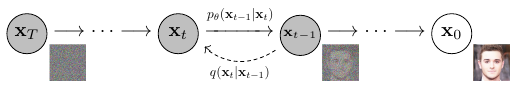
\includegraphics[width=12cm]{diffusion_Figure1.png}
\caption{Forward diffusion process $q$ and reverse diffusion model $p$.}
\end{figure}
Diffusion model is latent variable model 
$p_{\theta}(\rvx_0) = \int p_{\theta}(\rvx_{0:T}) d\rvx_{1:T}$ where the latents $\rvx_{1:T}$ have the same dims as the data $\rvx_0 \sim q(\rvx_0)$.
The joint distribution called the \emph{reverse process}\index{reverse process} is a Markov chain with learned Gaussian transitions
\begin{align*}
p_{\theta}(\rvx_{0:T}) = p(\rvx_T) \Pi_{t=1}^T p_{\theta}(\rvx_{t-1} \vert \rvx_{t}), \qquad p_{\theta}(\rvx_{t-1} \vert \rvx_{t}) = \mathcal{N}(\rvx_{t-1}; \mu_{\theta}(\rvx_t, t), \Sigma_{\theta}(\rvx_t, t))
\end{align*}

The diffusion process (\emph{forward process}\index{forward process}) is also a Markov chain adding gradually Gaussian noise to the data and is the approximate posterior of the model
\begin{align*}
q(\rvx_{1:T} \vert \rvx_0) = \Pi_{t=1}^T q(\rvx_{t} \vert \rvx_{t-1}), \qquad q(\rvx_{t} \vert \rvx_{t-1}) = \mathcal{N}(\rvx_{t}; \sqrt{1 - \beta_t}\rvx_{t-1}, \beta_t \mI) \enspace , 
\end{align*}
where $\beta_1, \ldots, \beta_T$ is a variance schedule.

Training is done by maximizing the usual variational lower bound on $\log p_{\theta}(\rvx_0)$ with the whole $\rvx_{1:T}$ as latent and using the Markov chain properties to decompose it into a sum of KL divergences over the chain conditionals $q(\rvx_{t} \vert \rvx_{t-1})$.
$\beta$'s can be trained by reparametrization trick or fixed as hyperparameters.

Interestingly, due to the specific formulation of the forward process, any timestep $t$ can be sampled using only the initial point $\rvx_0$ for conditioning 
\begin{align*}
q(\rvx_{t} \vert \rvx_0) = \mathcal{N}(\rvx_{t}; \sqrt{\bar\alpha_t}\rvx_{0}, 1-\bar\alpha_t \mI), \qquad \alpha_t = 1 - \beta_t, \ \bar\alpha_t = \Pi_{s=1}^t \alpha_s
\end{align*}
Due to this, the forward process Markov chain conditionals (the posteriors) are tractable when conditioned on $\rvx_0$
\begin{align*}
q(\rvx_{t} \vert \rvx_{t-1}, \rvx_0) = \mathcal{N}(\rvx_{t}; \bar\mu(\rvx_t, \rvx_0), \bar\beta_t \mI) \enspace ,
\end{align*}
where $\bar\mu$ is a fixed simple function of $\rvx_t, \rvx_0$ and some $\alpha$s and $\beta$s (see equation 7 in paper for details).

In their setup they do not learn $\beta$s but fix them - approximate posterior has no trainable parameters (no $\theta$s in the above), forward process is fixed.

The reverse process $p_{\theta}(\rvx_{t-1} \vert \rvx_{t}) = \mathcal{N}(\rvx_{t-1}; \mu_{\theta}(\rvx_t, t), \Sigma_{\theta}(\rvx_t, t))$ has in principal trainable mean and variance functions but they fix the variance to isotropic $\sigma_t \mI$ ($\sigma_t$ is a simple fixed function of $\beta_t$ - see paper).
With these the KL divergences in the ELBO loss can be evaluated in closed form (boil down to $\ell_2$ norms) and the only thing we learn are the mean functions $\mu_{\theta}(\rvx_t, t)$ of the $t-1$ step in the reverse process.

We can further reparametrize the sampling of $x_t$ by sampling the standard normal $\epsilon \sim \mathcal{N}(0, \mI)$ and $x_t = \sqrt{\bar\alpha_t}\rvx_{0} + \sqrt{1-\bar\alpha_t} \epsilon$ and hence $\rvx_0 = (\rvx_t - \sqrt{1-\bar\alpha_t} \epsilon) / \sqrt{\bar\alpha_t}$.
This does not seem very useful cause we do not learn any of the parameters. 
However, since by the loss the mean of the reverse process at step $t$ shall be the same as the mean of the forward process (which is obtainable in closed from from $\alpha$s and $\beta$s and the actual values of $\rvx$ generated by the forward process), we get that 
\begin{align*}
\mu_{\theta}(\rvx_t, t) = \frac{1}{\sqrt{\bar\alpha_t}}(\rvx_t - \sqrt{1-\bar\alpha_t} \, \epsilon_\theta(\rvx_t, t)) \enspace ,
\end{align*}
where $\epsilon_\theta(\rvx_t, t)$ is the function that shall be trained to minimize the ELBO.
To sample, we use $\rvx_{t-1} = \frac{1}{\sqrt{\bar\alpha_t}}(\rvx_t - \sqrt{1-\bar\alpha_t} \, \epsilon_\theta(\rvx_t, t)) + \sigma_t \rvz, \ \rvz \sim \mathcal{N}(0, \mI)$ recursively starting from $\rvx_t \sim \mathcal{N}(0, \mI)$ all the way back to $\rvx_0$.

With the introduction of $\epsilon$ the loss now resembles denoising score matching of \cite{song_generative_2020} and the sampling process the Langevin dynamics.

Nice experiments.












